%%%%%%%%%%%%%%%%%%%
%                                                        %
% SHPECK - SPECIATION MODEL  %
%                                                        %
%%%%%%%%%%%%%%%%%%%

\chapter{\emph{SHPECK} - Geochemical Speciation Model}
\label{chapter:SHPECK}

\emph{SHPECK} is a geochemical speciation model based on the \emph{Phase Rule} described in \cite{Garrels:65}. This is also the principle that is used in all of the speciation models reviewed in the previous section. 

As a computer simulation software, \emph{SHPECK} is a complete integrated model that allows: the user to set upchoosing; convert the chemical description to a system of equations; solving the system of equations; and present the results as graphical output.

This chapter will guide through all the aspects of the development of \emph{SHPECK} - a geochemical speciation modeling software. 

\section{Specification}
\emph{SHPECK} is a geochemical speciation modeling software designed to calculate the distribution of dissolved chemical elements as and aqueous solutes and complexes, and it also calculates saturation indexes for different minerals. 

\section{Architecture}
The architecture of the software is responsible for assuring that all the internal and external stakeholders' concerns are preserved, addressed and satisfied. The design of the architecture must occur prior the start of the development - it avoids waste of resources and re-work in the future. \emph{SHPECK}'s architectural design choices are done always to make sure that the software will bring value to the user.


Figure ~\ref{fig:shpeck-architecture} shows the software architecture of \emph{SHPECK}, which is modeled following the popular concept of \emph{Model-View-Controller} (MVC) \cite{Gamma:94}. \emph{MVC} is an architectural pattern that divides the software into three interconnected parts:
\begin{itemize}
\item Model: It is an object representing data or even activity. For example, the algorithm and math behind calculating the activity coefficient by Debye-Huckels' formula.
\item View: It is a form of visualization of the state of the model. For example, which are the solutes that the user wants to add into the simulation?
\item Controller: It offers facilities to change the state of the model. For example, define which algorithm for calculating the activity coefficient according to the user's choice or the value of the ionic strength (if the user did not specify which one to use).
\end{itemize}

\begin{figure}[ht!]
\centering
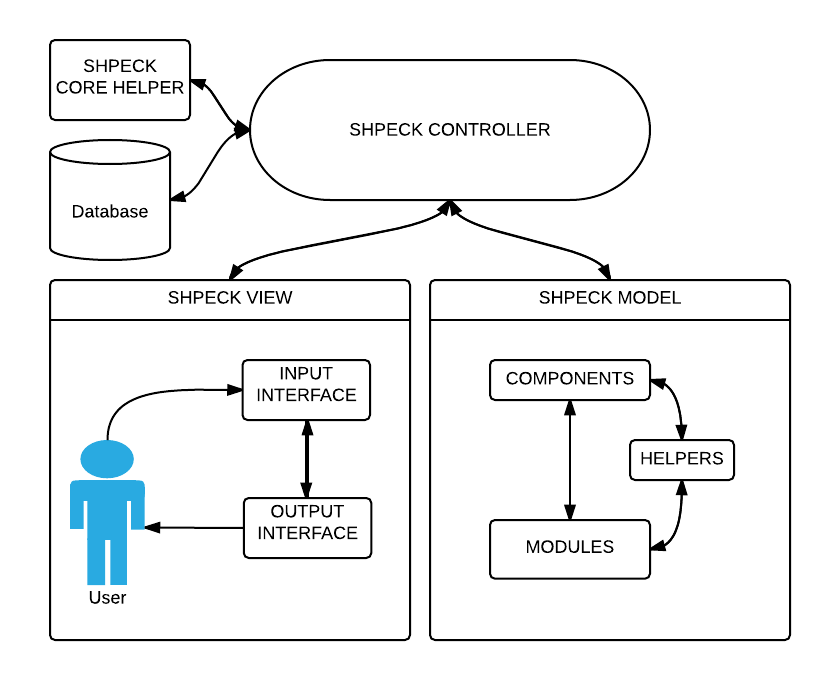
\includegraphics[width=100mm]{figures/shpeck-architecture.png}
\caption{Architecture of the \emph{SHPECK} software}
\label{fig:shpeck-architecture}
\end{figure}

\subsection{Technical Specification}
\emph{SHPECK} is a software developed using C++, which is a general-purpose programming language. C++ has a bias toward system programming that supports efficient low-level computation, data abstraction, object-oriented programming, and generic programming \cite{Dale:04} \cite{Stroustrup:97}. It provides powerful and flexible mechanisms for abstraction. In other words, the language allows the programmer to introduce and use new types of objects that match the concepts of an application needed. Thus, C++ supports styles of programming that rely on relatively direct manipulation of hardware resources to deliver a high degree of efficiency. It can also address higher-level styles of programming that rely on user-defined types to provide a model of computation that is closer to human's view of the task being performed by a computer. Application libraries often support these higher level styles of programming. While developing Shpeck, two supporter tools were adopted:
\begin{itemize}
\item \emph{Qt} : It is a cross-platform application and UI framework for developers using C++  \cite{Qt:14}. \emph{Qt} turns the development fast and easy. with extensive built-in library classes available, it provides a comprehensive range of functionality, as well as a convenient platform.
\item \emph{Armadillo} : It is a C++ linear algebra library that provides classes for vectors, matrices, cubes and a whole set of functions to operate on the classes \cite{arma:14}. With a syntax of the library is similar to Matlab, and an up-to-date support with upgrades and new releases are available  on monthly basis.
\end{itemize}
Important to mention that the system is being developed using \emph{MAC} but since the beginning of the development process, the goal is to develop a multi-platform software to be distributed either in \emph{Windows} and \emph{LINUX-like} systems.

\section{Governing equations}
%These chemical equations represent the mathematical model that drives the methods that are executed in \emph{SHPECK}. Their behavior defines the steps and the order in which they are presented. This set of equations models a real-world system and is named \emph{computer simulation model}.

\emph{SHPECK} uses thermodynamic equilibrium reactions as equations for the calculation of multiphase systems in equilibrium. Details and treatments of these reactions are discussed in details in chapter ~\ref{chapter:basic}. A set of mass-action equations (as in equation ~\ref{eq:massaction}) compose the system, and the number of species and compounds that coexist in the system defines the number of equations. These equations model the geochemical speciation in a closed system taking into account the chemical properties of the solutes.

Aside from the mass-action equations there must be additional constraints to solve the equilibrium state of the system. In \emph{SHPECK}, I use the concentration of the species to deal with the equilibrium state of the system. Therefore, I have the following configuration:

\begin{equation}\label{eq:configuration}
S_{aqueous} = N_{reactions} + N_{eq constraints}
\end{equation}

where $S_{aqueous}$ are the number of aqueous solutes in the solution, $N_{reactions}$ are the number of mass-action equations and $N_{eq constraints}$ are the number of equilibrium constraints imposed by the user. 
In order to have a better efficiency on the method, we use equation ~\ref{eq:massactionLog} reformulated by applying natural logarithm in both sides, as expressed below:
\begin{equation}\label{eq:massactionLog}
ln({K_j}) =  ln({\prod\limits_{i=1}^N  a_i^{v_{ij}}}) \hspace{35pt}    (j = 1, ... , M)
\end{equation}

\section{Numerical Method}
In order to solve the system composed of the equilibrium state of the mass-action equations and the equilibrium constraints, \emph{SHPECK} uses a numerical method that solves the complete set of equations simultaneously and find the value of the unknowns (solute concentrations).


The numerical method applied is a modification of the \emph{Newton's method} (also known as Newton-Raphson method), which is a method for finding successively better approximations to the roots of the given set of equations. It works with a derivative approach to the equations, which optimizes the time consumed to find the roots and makes the representation of the system easier.

\emph{SHPECK} uses the \emph{Newton-Raphson} method to solve a nonlinear system of equations which results in finding the roots of continuously differentiable equations. 

The \emph{Newton-Raphson} method is applied in order to achieve the best approximation possible to the solution that is being sought. It is an iterative algorithm where each step consists in minimizing the first-order approximation of the solution. \emph{Newton-Raphson} method is a modification of \emph{Newton}'s method for finding a minimum of a function. Its difference from regular \emph{Newton}'s method is that second derivatives are not required. \emph{Newton-Raphson}'s method is used to solve a system of coupled nonlinear equations. The first-order approximation of the function starts with an initial guess for the minimum values, the method proceeds by the iterations as shown in equations ~\ref{eq:NewtonMethodEq1}.

\begin{equation}
\label{eq:NewtonMethodEq1}
F(x+1) = F(x) - J^{-1} * R
\end{equation}

Where $F$ is function's result for the applied $x$, $J^{-1}$ is the inverse of the Jacobian matrix, and $R$ is the residual vector \cite{Isaacson:66}.

The \emph{Jacobian Matrix} receives the equations and generates a model that does it automatically. The \emph{Jacobian Matrix} is the matrix of all first-order partial derivatives of the equation and it is defined as

\begin{equation}
\label{eq:JacobianDefinition}
J_{mn} = \frac{\partial y^m}{\partial x^n}
\end{equation}

where the $y^i$'s are a new coordinate system defined in terms of the original coordinate system, the $x^i$'s. In differential equation theory, the Jacobian matrix plays a key role in defining the stability of solutions.

The $R$ residual vector is defined as a vector containing the resulting values for each equation.

\begin{equation}
\label{eq:residualVector}
R = \begin{pmatrix}
 F(x_1) \\
 \vdots \\
 F(x_m)
 \end{pmatrix}
\end{equation}

Where $m$ is the number of unknowns (or mass-action equations plus equilibrium constraints).

The algorithm consists of iteratively calculating new approximations for the unknown values, through the matrix equation:

\begin{equation}
\label{eq:iterativelyAlgorithm}
[J]^{-1}_{iteration}* \alpha [U]_{iteration+1} = [R]_{iteration}
\end{equation}

Where $J$ is the Jacobian Matrix; $ \alpha [U]_{iteration+1} $ is the unknown composition at the next iteration; iteration is the iteration number and $R$ is the residual matrix. With this, it is possible to state the $[U]_{iteration+1}$ value with:

\begin{equation}
\label{eq:CompositionCalculation}
[U]_{iteration+1} = [U]_{iteration} + \alpha [U]_{iteration+1}
\end{equation}


The initial guess of the solutions is an approximation that the user provides to the \emph{Newton-Raphson} method. This method needs a \emph{seed} to start the calculations (usually this guess is used for $F(0)$). 
If the guess is close to the real root value the number of iterations necessary to obtain the solution is small. If the guess is far from the real solution, more iterations are needed to find the correct solution.

Specifically, \emph{SHPECK}'s equations can be described as: $F_1(x_1,..., x_n)$,...,$F_m(x_1,...,x_n)$. The partial derivatives of all these equations with respect to the variables $x_1,...,x_n$ can be organized in a m-by-n matrix, the Jacobian matrix, as bellow:

\begin{equation} 
J =
 \begin{pmatrix}
  \frac{\partial F_1}{\partial x_1} & \cdots & \frac{\partial F_1}{\partial x_n} \\
  \vdots  & \ddots & \vdots  \\
  \frac{\partial F_m}{\partial x_1} & \cdots &   \frac{\partial F_m}{\partial x_n}
 \end{pmatrix}
\end{equation}

In our case, $m = n$ and the \emph{jacobian matrix} is a square matrix and is generated once. With the equations selected and organized, the derivatives of each reaction towards each variable are calculated and the \emph{jacobian matrix} is modeled and stored. 

It is important to realize that the main complication of using the \emph{Newton-Raphson} method to solve a system of nonlinear equations is defining the functions included in the \emph{Jacobian Matrix}. As the number of equations and unknowns increases (n), so does the number of elements in the \emph{Jacobian} ($n^2$).
\section{Algorithm}

\emph{SHPECK}'s algorithm takes as its input a specification of the system's state. For example, this consists of the values for the concentrations of the solutes in the solution, the temperature of the system, the method used to calculate activity coefficient, etc. It then calculates the system's state by executing the numerical iterative process of achieving a solution. 
Figure ~\ref{fig:Shpeck-algo} presents the high-level algorithm in details. It is important to understand that each of the boxes in this algorithm represents a set of instructions, calculations, and conditional clauses. Due to this work's scope we only specify the algorithm inside the box called "Newton's Method Solver". The algorithm of how the governing equations control the numerical methods is presented in figure ~\ref{fig:Shpeck-algo-newton}. 
\begin{figure}[ht!]
\centering
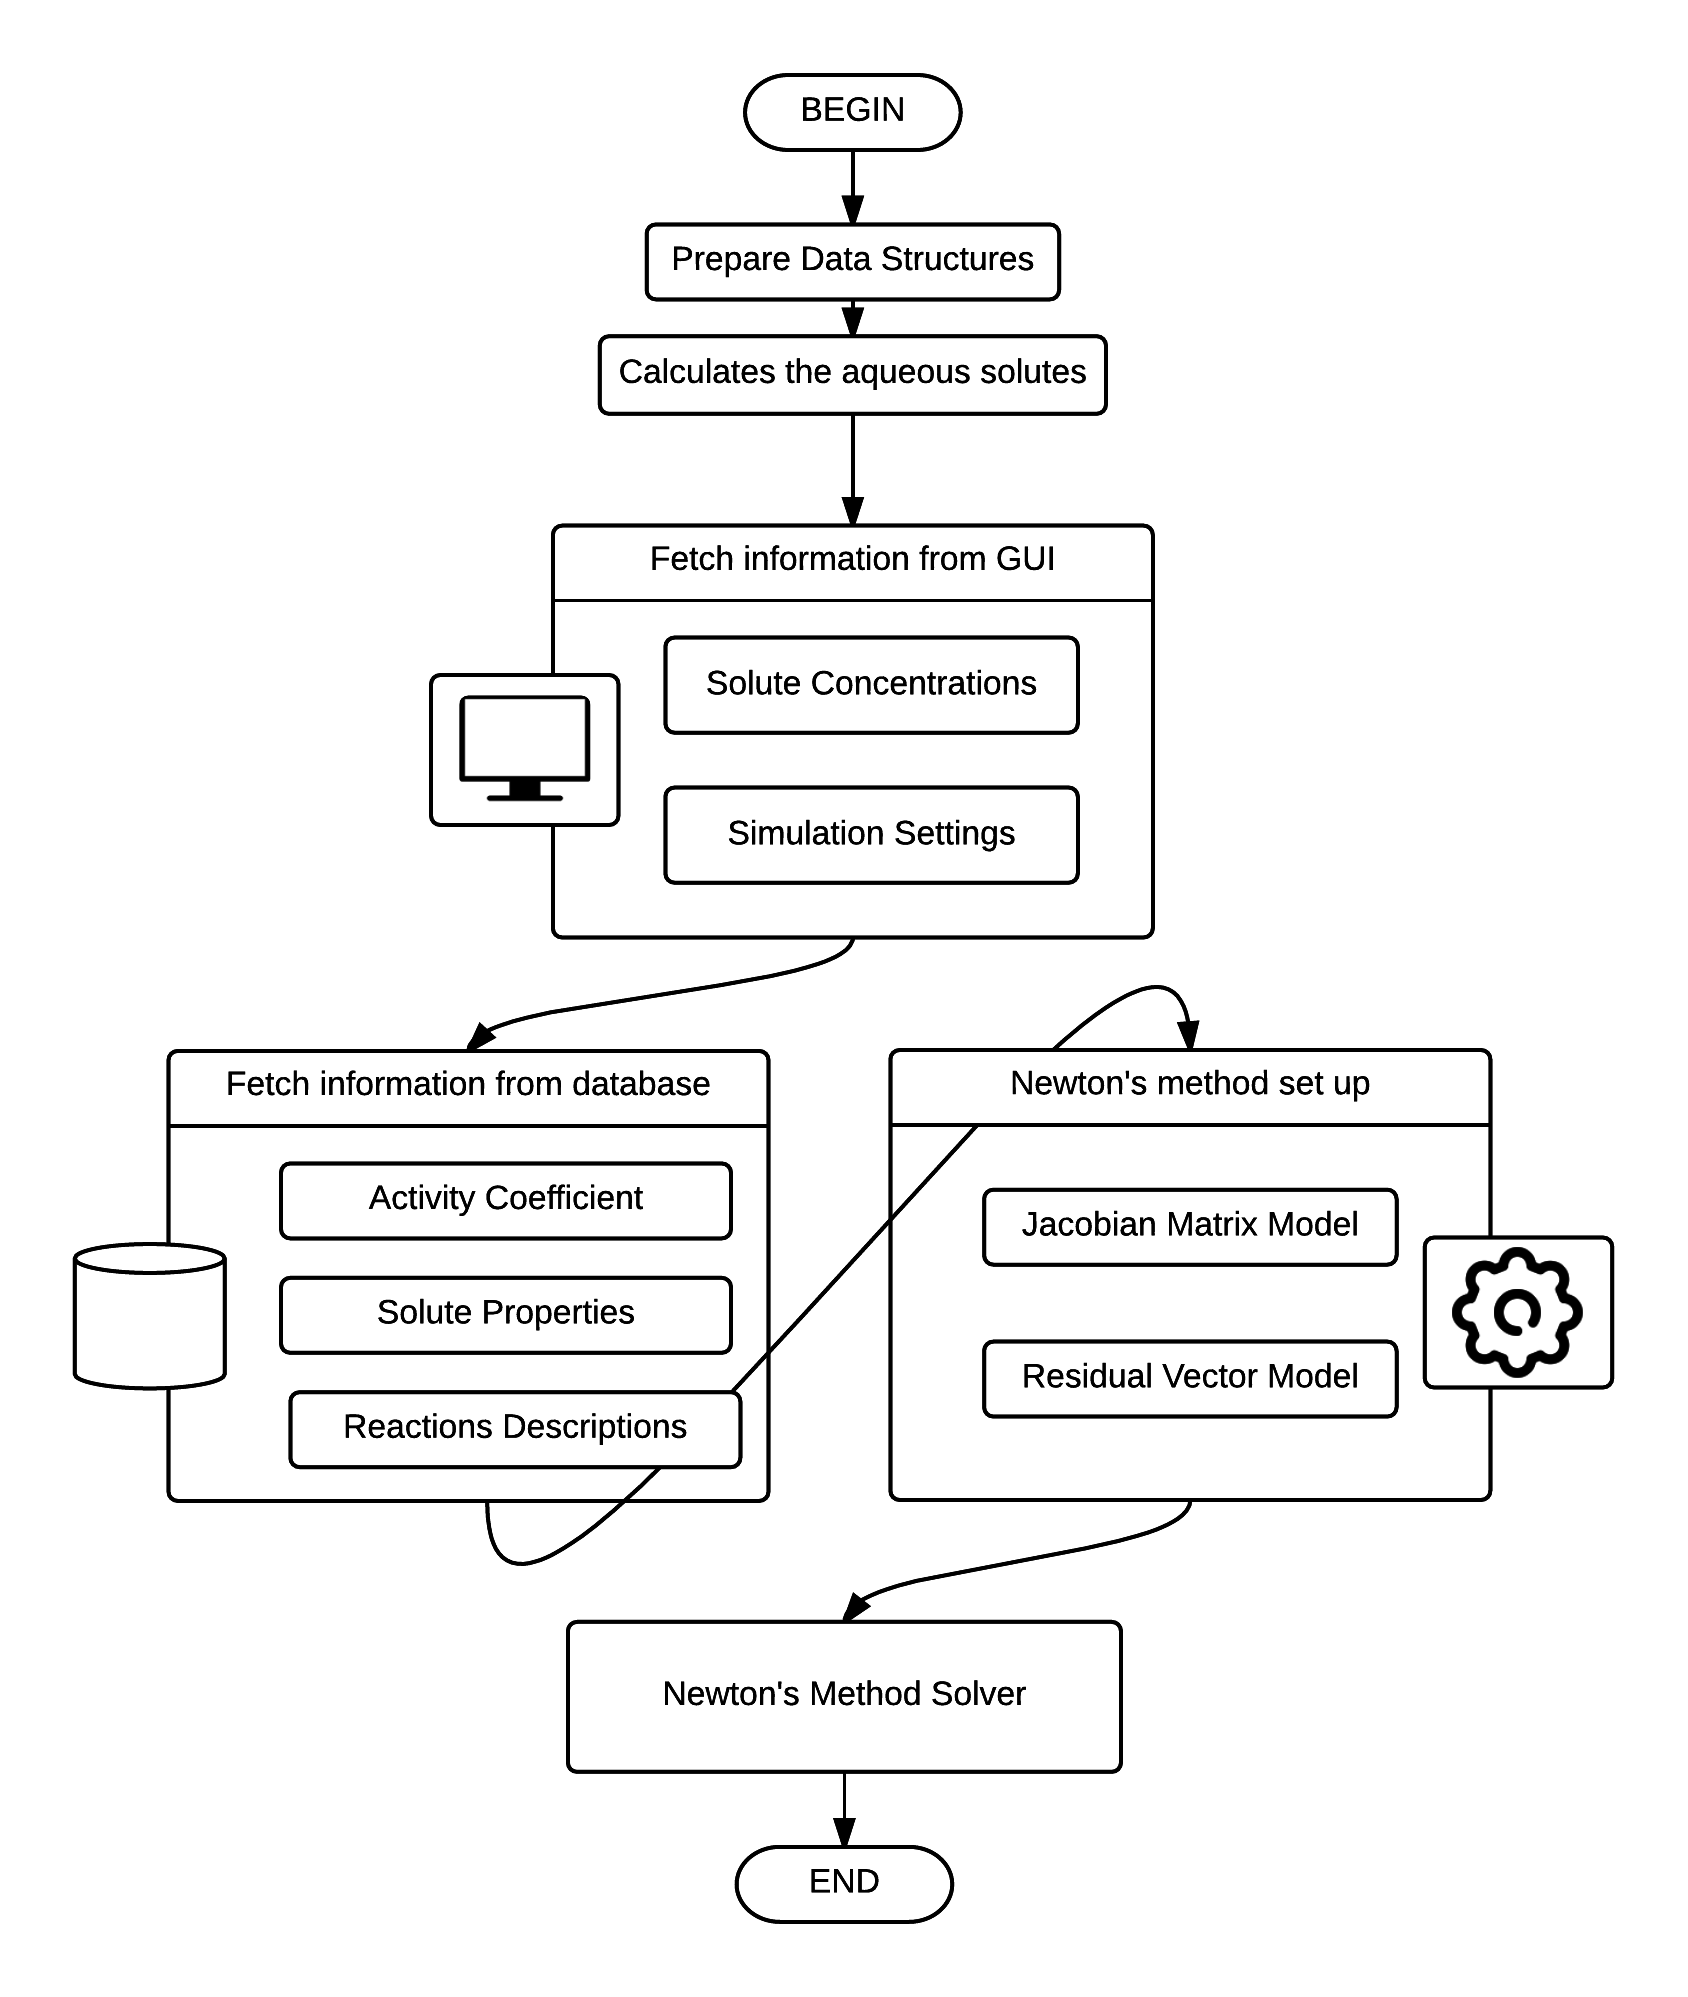
\includegraphics[width=100mm]{figures/Shpeck_algo3.png}
\caption{High-level algorithm of \emph{SHPECK}}
\label{fig:Shpeck-algo}
\end{figure}
\begin{figure}[ht!]
\centering
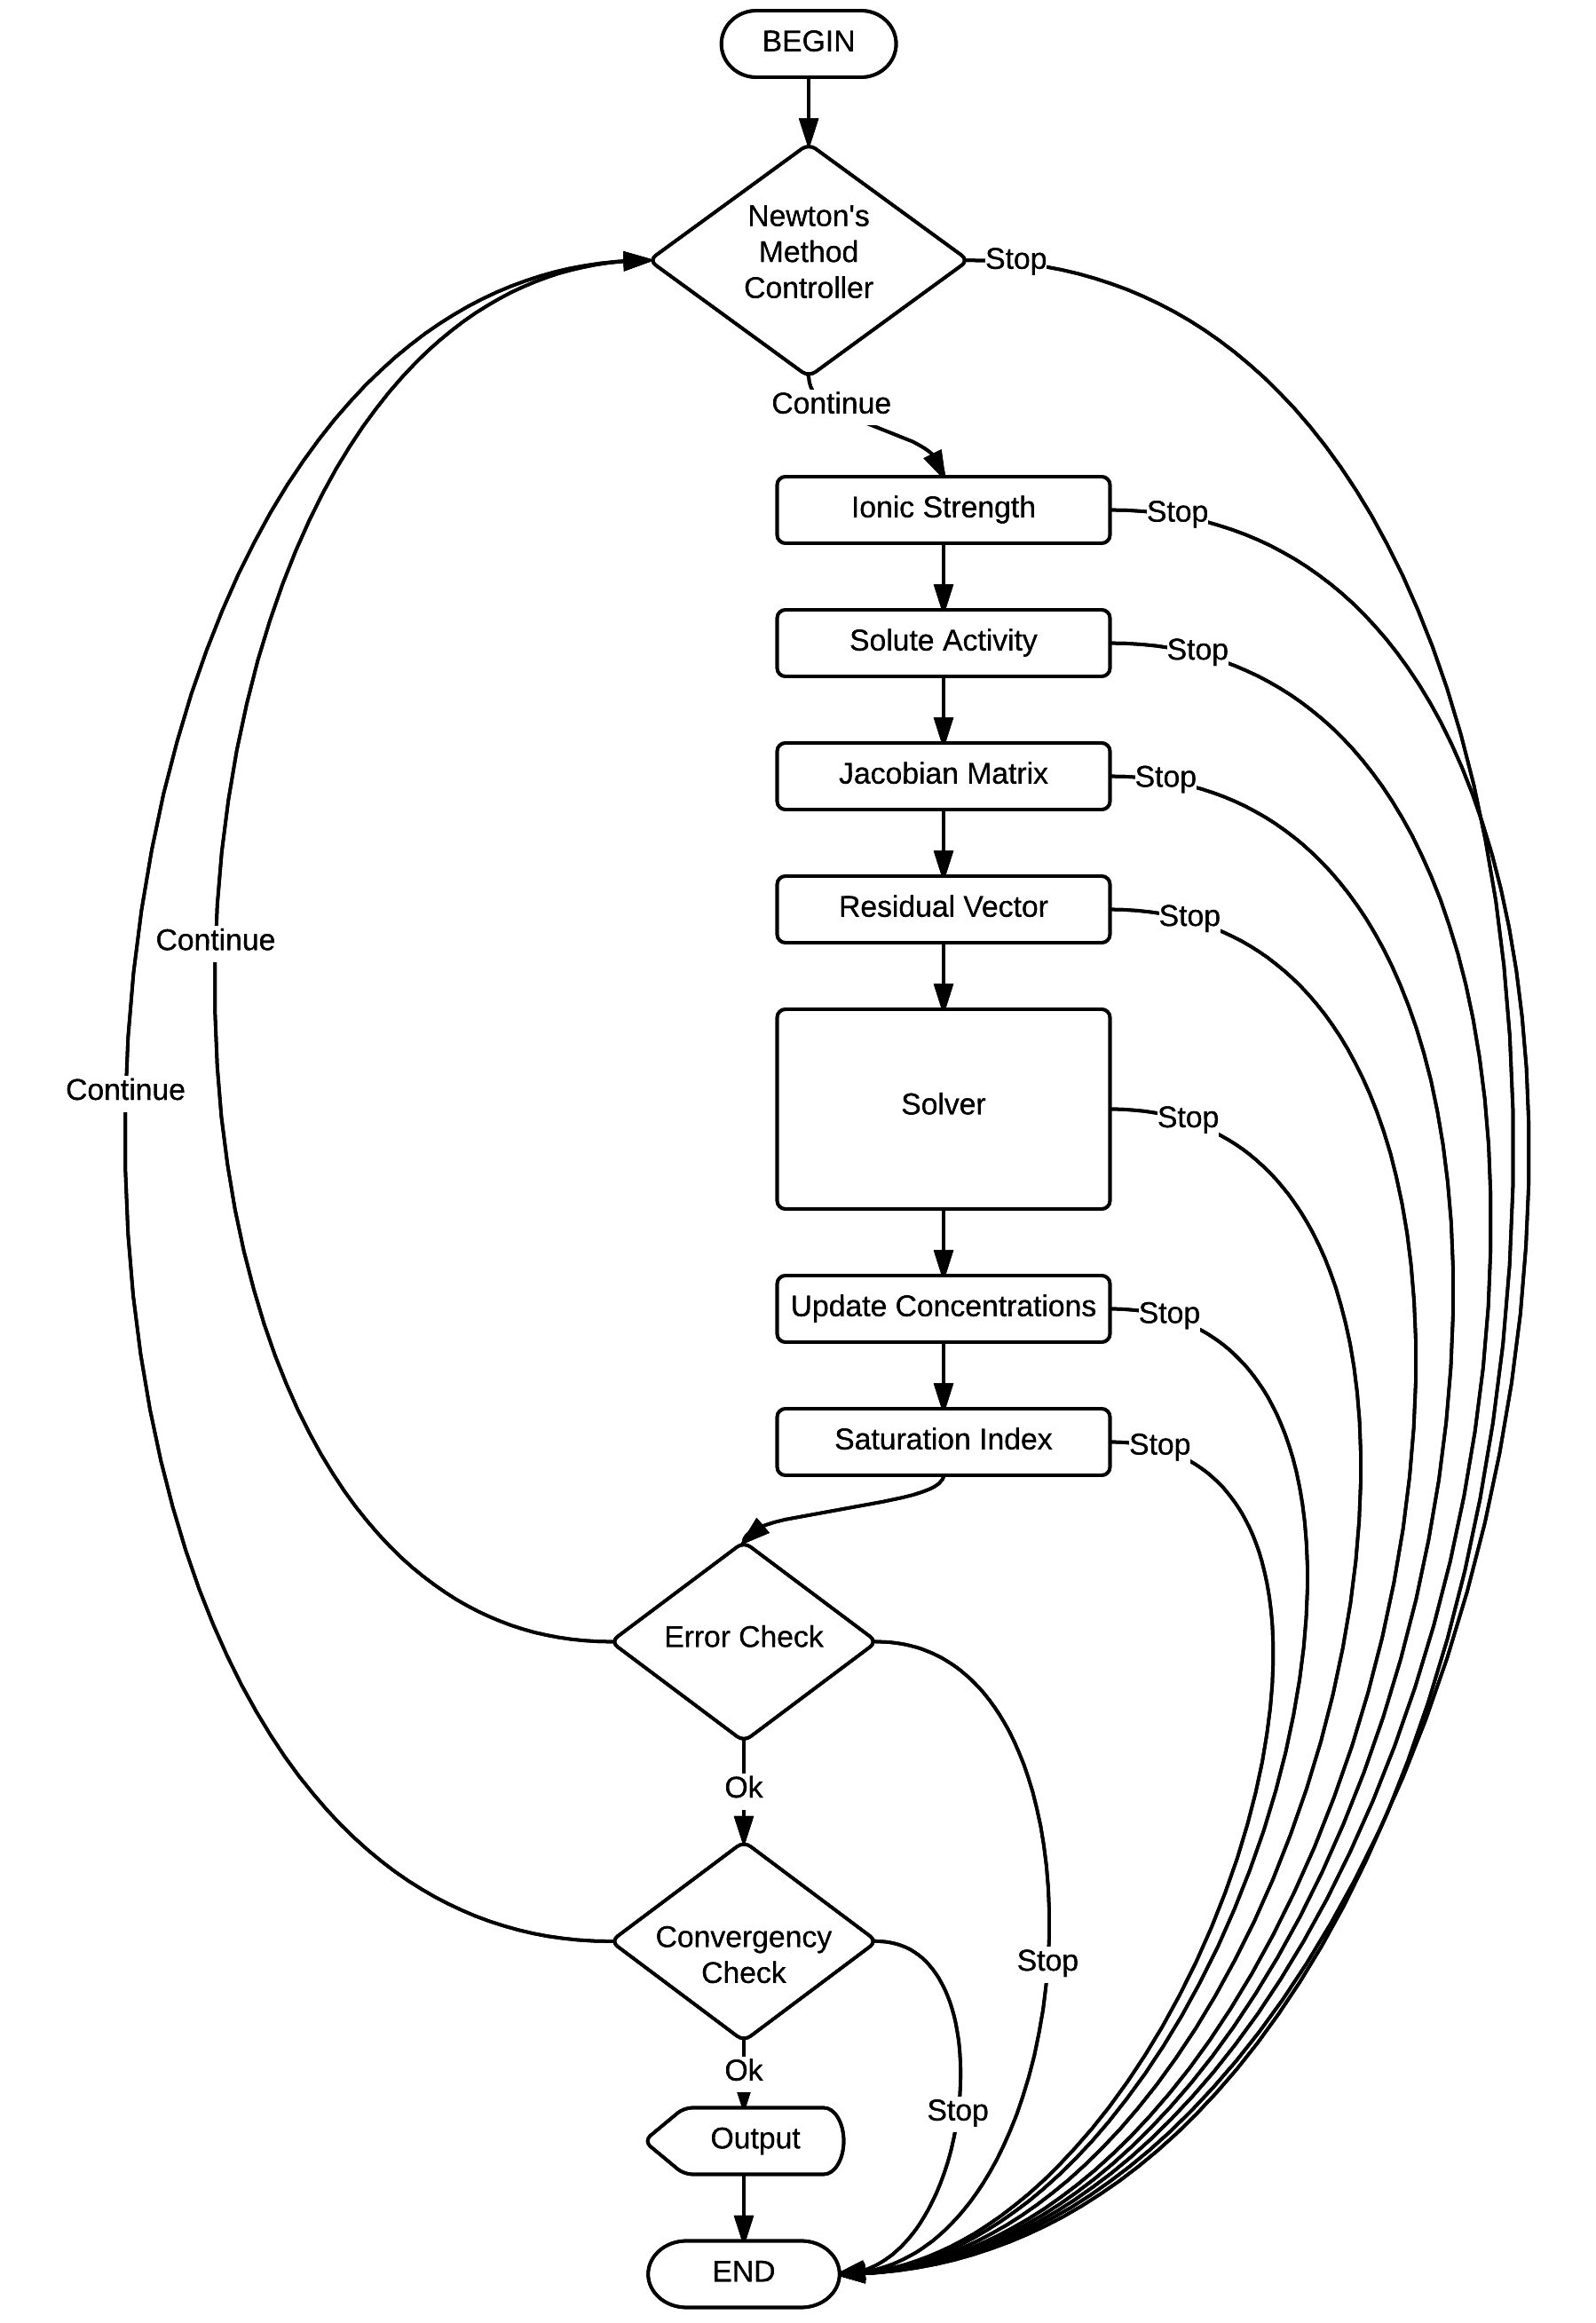
\includegraphics[width=100mm]{figures/Shpeck_algo_newton.png}
\caption{Algorithm of the Newton's Method Solver}
\label{fig:Shpeck-algo-newton}
\end{figure}
\subsection{Complexity of the algorithm}
The \emph{Newton-Raphson}'s method has a complexity O($n^3$) per iteration with a quadratic convergence.

%(http://ranger.uta.edu/~huber/cse4345/Notes/Nonlinear_Equations.pdf)
%(http://ranger.uta.edu/~huber/cse4345/Notes/Equations.pdf)
%(compared to http://en.citizendium.org/wiki/Newton%27s_method#Computational_complexity)


\section{Graphical User Interface}
Due to the enormous amount of options connected to the nature of geochemical modeling, it is necessary to develop the software as an intuitive and user-friendly utility. The development of the GUI introduces several stages of processes related to it:
\begin{itemize}
\item Planning : This moment is where the developer needs to conceptualize and evaluate the options toward constructing the core of the program that is intuitive and friendly to the user. The planning is an essential process. The content, features, and details of the software need to be strictly defined and organized. There is a small gap from an useful software from one that is not useful at all. Especially, guessing the role of a user is a difficult task, simply because the developer is not the final user for its applications. It is important also to find out if there are comparable software already in the public domain.
\item Building : The planning for the implementation of the features of the software is important to be well defined at this point. To build the tool \emph{Qt} - already presented above - was chosen due to its many advantages, since it is easy to customize, no coding was necessary, templates are available, provides a simple drag and drop \emph{GUI}  builder, and is secure and reliable;
\item Ensuring Usability : The challenge in the field of Human-Computer Interaction (HCI) investigates the way in which people use computers. Techniques and tools are used to find relevant standards. These include tests with real users, evaluation by experts, gathering user feedback, and usage logging;
\end{itemize}


\subsection{\emph{SHPECK}'s GUI }
In existing geochemical modeling software the GUI are either poorly implemented, or not implemented at all. We see\emph{SHPECK} as geochemical speciation modeling software with a potential to broaden its influence. The \emph{GUI} enables the user to streamline and conveniently construct a geochemical environment for modeling.
\emph{SHPECK}'s \emph{GUI} works based on tabs. Each tab is responsible for viewing a specific point of the software. I present them in detail below:
\begin{itemize}
\item Configurations tab: This allows users to view and manipulate basic system settings and controls such as temperature, activity coefficient calculation method, the number of iterations, solver options, and error and convergence criteria. It is presented in ~\ref{fig:config}.
\item Compounds in the water tab: Allows users to create and edit the composition of the water that will be used in the geochemical speciation model. It has the complete catalog of species available from the database. The species in the tab that have concentrations other than zero compose the water. This tab is presented in ~\ref{fig:water}.
\item Results tab: Allows the user to see relevant input information and the outputs of the geochemical speciation model such temperature, ionic strength, pH of the solution, final concentration for the species, saturation indexes, etc. It is presented in ~\ref{fig:output}.
\end{itemize}


\begin{figure}[ht!]
\centering
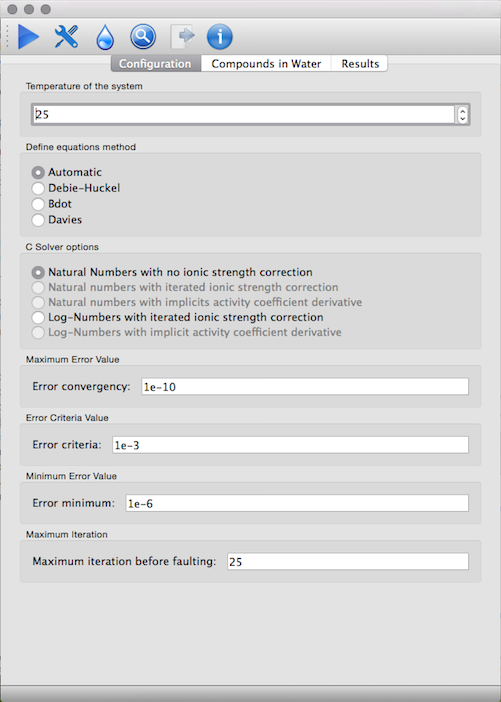
\includegraphics[width=100mm]{figures/shpeck-configtab.png}
\caption{Configuration tab}
\label{fig:config}
\end{figure}

\begin{figure}[ht!]
\centering
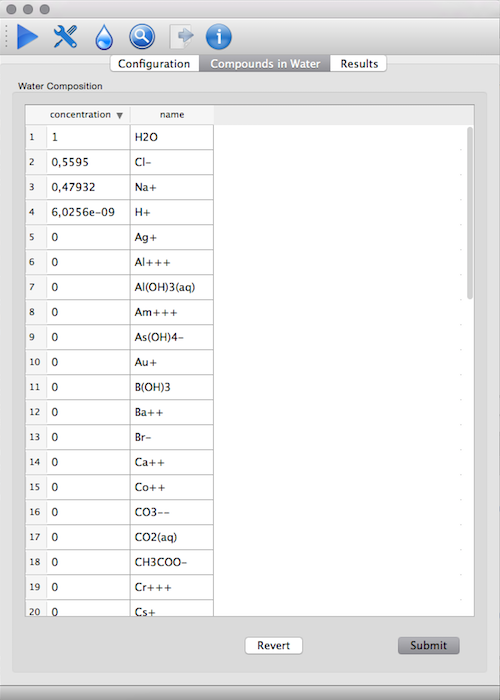
\includegraphics[width=100mm]{figures/shpeck-watertab.png}
\caption{Water composition tab}
\label{fig:water}
\end{figure}

\begin{figure}[ht!]
\centering
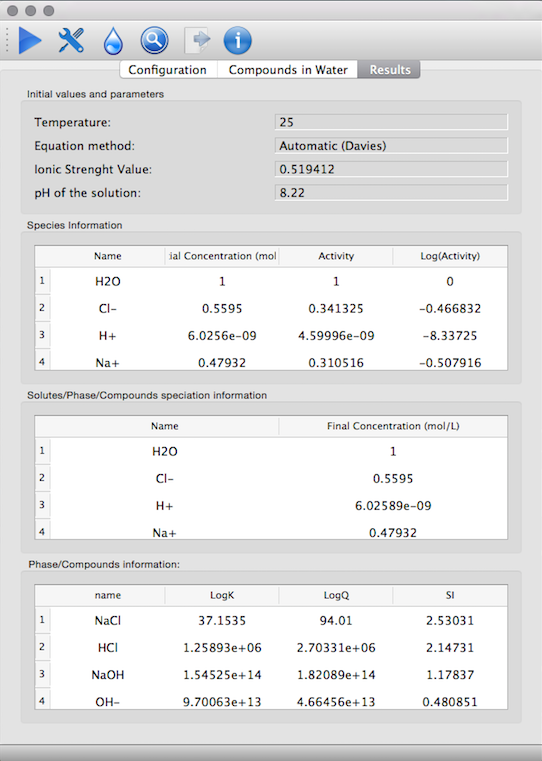
\includegraphics[width=100mm]{figures/shpeck-resultstab.png}
\caption{Results tab}
\label{fig:output}
\end{figure}

\section{Database}
As can be seen in this chapter, the algorithm of \emph{SHPECK} is not trivial and requires many interactions between many different entities. The database is responsible for providing the data that will flow through and works as the \emph{seed} provider. Chapter ~\ref{chapter:review} makes clear that using a flat file database poses difficulties to users. Potential issues of using flat file databases are: duplication of the information; non-unique records; difficulty in updating and maintenance; inherently inefficient; rigid (difficult data format); and insecure.
In \emph{SHPECK}, we use a relational database, which is a model of a database that prevents all the problems faced in flat file database previously discussed. A relational database works based on a \emph{query}, which is an information request from the database. Besides that, there are three important advantages:
\begin{itemize}
\item A relational database has another advantage of the content existing as an external entity to the memory allocated by the software. Also, these databases are often larger than the computer's RAM capacity. By using a database system, the software fetches the information on-the-go. 
\item Complex queries enable the versatility and efficiency when fetching relevant information from the database. Instead of scanning through flat files, the query can pre-define the categories of information - even from multiple tables - that will be sought. Also important to mention, a query can be composed and concatenated on runtime execution - meaning that \emph{SHPECK} only fetches from the database information relevant to the specific simulation that is being executed (species, compounds, reactions, etc.). Complex queries and concatenation of queries result in a faster and more efficient use of the available resources.
\end{itemize}

The database is one of the most critical and significant infrastructure component of our software. The database architecture was defined after studying the algorithm and determining the structure and the information that will be needed - this is presented in detail in figure ~\ref{fig:ERDiagram}. We developed a relational database that incorporates the data already in use from other software, but with a newer approach and organized as structured tables. Naturally, some changes in the structure were necessary in order to derive a more relevant database for the software.

\begin{figure}[ht!]
\centering
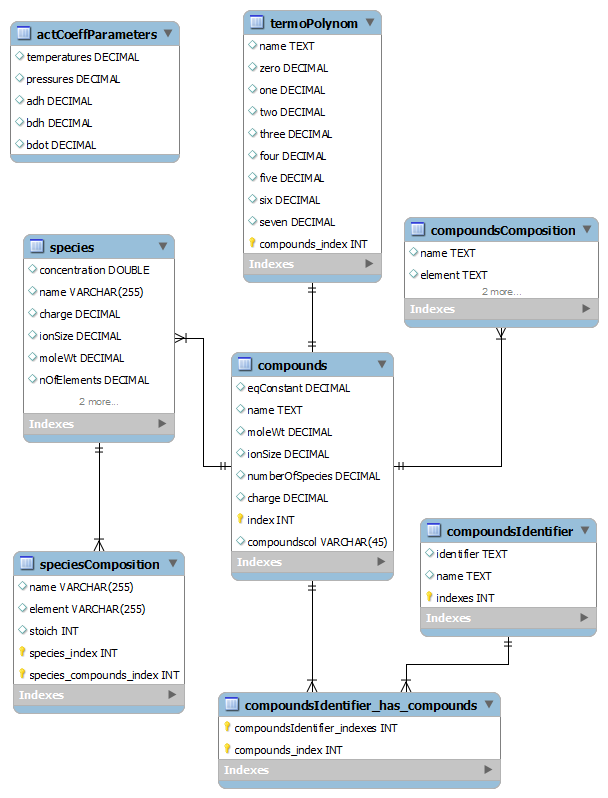
\includegraphics[width=100mm]{figures/ER_diagram.png}
\caption{ER Diagram of the database}
\label{fig:ERDiagram}
\end{figure}

\subsection{Database Technologies}
We use the SQLite database \cite{SQLite}, which is a software library that implements a self-contained, transactional \emph{SQL} database engine, open source and currently is the most widely deployed \emph{SQL} database engine in the world. Some of its advantages are explained bellow:
\begin{itemize}
\item Zero-Configuration: \emph{SQLite} does not need to be installed before it is used, there is no setup procedure;
\item Serverless: The process that wants to acess the database reads and writes directly from the database files on disk. There is no intermediary server process (nor interprocess communication using \emph{TCP/IP});
\item Single Database File: An \emph{SQLite} database is a single file located in the directory hierarchy. \emph{SQLite} database can be easily copied onto a USB memory stick or emailed for sharing;
\item Stable Cross-Platform Database File: A database file written on one machine can be copied and used on a different machine with a different architecture. Furthermore, \emph{SQLite} is backwards compatible (newer versions can read and write older database files);
\end{itemize}

\subsection{\emph{LLNL} thermodynamic dataset parser}
Once the structure and the technology of our database were defined, a parser was prepared to extracted the information from the flat file database. 
The parser was generated carefully in order to ensure that all of the data and delimiters were identified and treated properly. This task was extremely time-consuming because of irregularities found in the flat files.

\newpage

\section{Summary}
\begin{itemize}
\item Architecture: \emph{SHPECK} follows the architectural pattern called \emph{MVC}; Its benefits are the complete separation of responsibilities and concerns among the parts of the software. Thus, there is no mixing of codes between them. Another advantage is its flexibility that allows the software to grow and develop further. Figure ~\ref{fig:shpeck-architecture} displays the \emph{MVC} pattern existing in \emph{SHPECK}.
\item Governing Equations: \emph{SHPECK} is a geochemical speciation modeling software that drives the behavior of the aqueous system based on a set of mass-action equations combined with equilibrium constraints. A mass-action equation is described in equation  ~\ref{eq:massaction} and reinforced here:

\begin{equation}
K_j =  \prod\limits_{i=1}^N  a_i^{v_{ij}} \hspace{35pt}    (j = 1, ... , M)
\end{equation}

where $K_j$ denotes the equilibrium constant of the \emph{j-th} reaction; $a$ denotes the activity of the \emph{i-th} chemical species.

\item Numerical Method: \emph{SHPECK} applies the \emph{Newton-Raphson} method to solve the nonlinear system of equations. The concept of the method is described in equation ~\ref{eq:NewtonMethodEq1} and reinforced here:

\begin{equation}
F(x+1) = F(x) - J^{-1} * R
\end{equation}

Where $F$ is function's result for the applied $x$, $J^{-1}$ is the inverse of the Jacobian matrix, and $R$ is the residual matrix. The quadratic rate of convergence of this method compensate the expensive calculation inherent to it.

\item Graphical User Interface: The \emph{GUI} mission is to enable the user to use the full potential \emph{SHPECK} has to offer. It is intuitive and user-friendly to allow the user to focus on essential duties that are imperative to modeling a geochemical environment. We use the popular approach of \emph{tab} panels, which are separated according to their purposes: configurations and settings, water composition, and results visualization.
\item Database: A geochemical modeling software is dependent on the information provided in the database. \emph{SHPECK} structures all of its data in a \emph{SQLite} relational database, which is unique approach among the comparable software available. \emph{SHPECK}'s database is composed of the information on elements, species, compounds, reactions and thermodynamic constants found in the \emph{LLNL} thermodynamic dataset. A parser for \emph{LLNL} flat file database was created to fetch this information.
\end{itemize}